\documentclass[11pt]{article}
\usepackage{amsmath}
\usepackage{caption}

\usepackage{algorithmicx}
\usepackage{algpseudocode}
\usepackage{algorithm}

\usepackage{graphicx}
\usepackage{listings}

\title{Exercisesheet No.1}
\author{Alexander Diete \and Magnus M\"uller \and Martin Pfannem\"uller}

\begin{document}
\maketitle
\section*{Ex.1}
$$(((P \vee Q) \Rightarrow R) \wedge (R \vee (P \wedge \neg Q))) \wedge \neg R$$
Translate the implication to an or-clause:
$$((\neg(P \vee Q) \vee R) \wedge (R \vee (P \wedge \neg Q))) \neg R$$
De Morgan:
$$(((\neg P \wedge \neg Q) \vee R) \wedge (R \vee (P \wedge \neg Q))) \wedge \neg R$$
Distributivity:
$$((\neg P \vee R) \wedge (\neg Q \vee R) \wedge (R \vee P) \wedge (R \vee \neg Q))\wedge \neg R$$
Distributivity (inverse):
$$(R \vee (\neg P \wedge \neg Q \wedge P \wedge \neg Q))\wedge \neg R$$
Complements over P ($(\neg P \wedge \neg Q \wedge P \wedge \neg Q) = $false):
$$R \wedge \neg R$$

We are ending up with a contradiction.

\section*{Ex.2}

$\displaystyle Init(Room(Room1) \wedge Room(Room2) \wedge Room(Room3) \wedge Room(Room4) \wedge Room(Corridor) \wedge Switch(s1) \wedge Switch(s2) \wedge Switch(s3) \wedge Switch(s4) \wedge Box(b1) \wedge Box(b2) \wedge Box(b3) \wedge Box(b4) \wedge Door(Door1) \wedge Door(Door2) \wedge Door(Door3) \wedge Door(Door4) \wedge At(Shakey,Floor) \wedge In(Shakey,Room3) \wedge TurnedOn(s4) \wedge TurnedOff(s3) \wedge TurnedOff(s2) \wedge TurnedOn(s1) \wedge In(b1,Room1) \wedge In(b2,Room1) \wedge In(b3,Room1) \wedge In(b4,Room1) \wedge At(s1,Room1) \wedge At(s2,Room2) \wedge At(s3,Room3) \wedge At(s4,Room4) \wedge In(Door1,Room1) \wedge In(Door1,Corridor) \wedge In(Door2,Room2) \wedge In(Door2,Corridor) \wedge In(Door3,Room3) \wedge In(Door3,Corridor) \wedge In(Door4,Room4) \wedge In(Door4,Corridor))$

\begin{lstlisting}[mathescape=true]
Action(Go(x,y,r)),
  PRECOND: $At(Shakey, x) \wedge In(x,r) \wedge In(y,r)$
  EFFECT: $At(y,Shaky) \wedge \neg At(x,Shaky)$

Action(Push(b,x,y,r)),
  PRECOND: $At(b,x) \wedge In(x,r) \wedge In(y,r) \wedge In(Shakey,r) \wedge \neg At(Shakey,x) \wedge Box(b)$
  EFFECT: $At(b,y) \wedge \neg At(b,x)$  
  
Action(ClimbUp(x,b)),
  PRECOND: $In(b,r) \wedge In(x,r) \wedge At(Shakey,x) \wedge \neg At(b,x) \wedge On(Shakey, Floor)$
  EFFECT: $\neg On(Shakey, Floor) \wedge On(Shakey, b) \neg At(Shakey, x)$  

Action(ClimbDown(b,x)),
  PRECOND: $In(x,r) \wedge In(b,r) \wedge \neg At(b,x) \wedge On(Shakey, b)$
  EFFECT: $\neg On(Shakey, Floor) \wedge On(Shakey, b) \neg At(Shakey, x)$
  
Action(TurnOn(s,b)),
  PRECOND: $On(Shakey,b) \wedge \neg On(Shakey,Floot) \wedge At(b,s) \wedge At(Shakey, s)$
  EFFECT: $TurnedOn(s)$

Action(TurnOff(s,b)),
  PRECOND: $On(Shakey,b) \wedge \neg On(Shakey,Floot) \wedge At(b,s) \wedge At(Shakey, s)$
  EFFECT: $TurnedOff(s)$

Plan:
Go(X,Door3,Room3)
Go(Door3,Door1,Corridor)
Go(Door1,Box2,Room1)
Push(Box2,Box2,Door1,Room1)
Push(Box2,Door1,Door2,Corridor)

\end{lstlisting}

\section*{Ex.3}

See figure \ref{fig:3}.

\begin{figure}
	\centering
  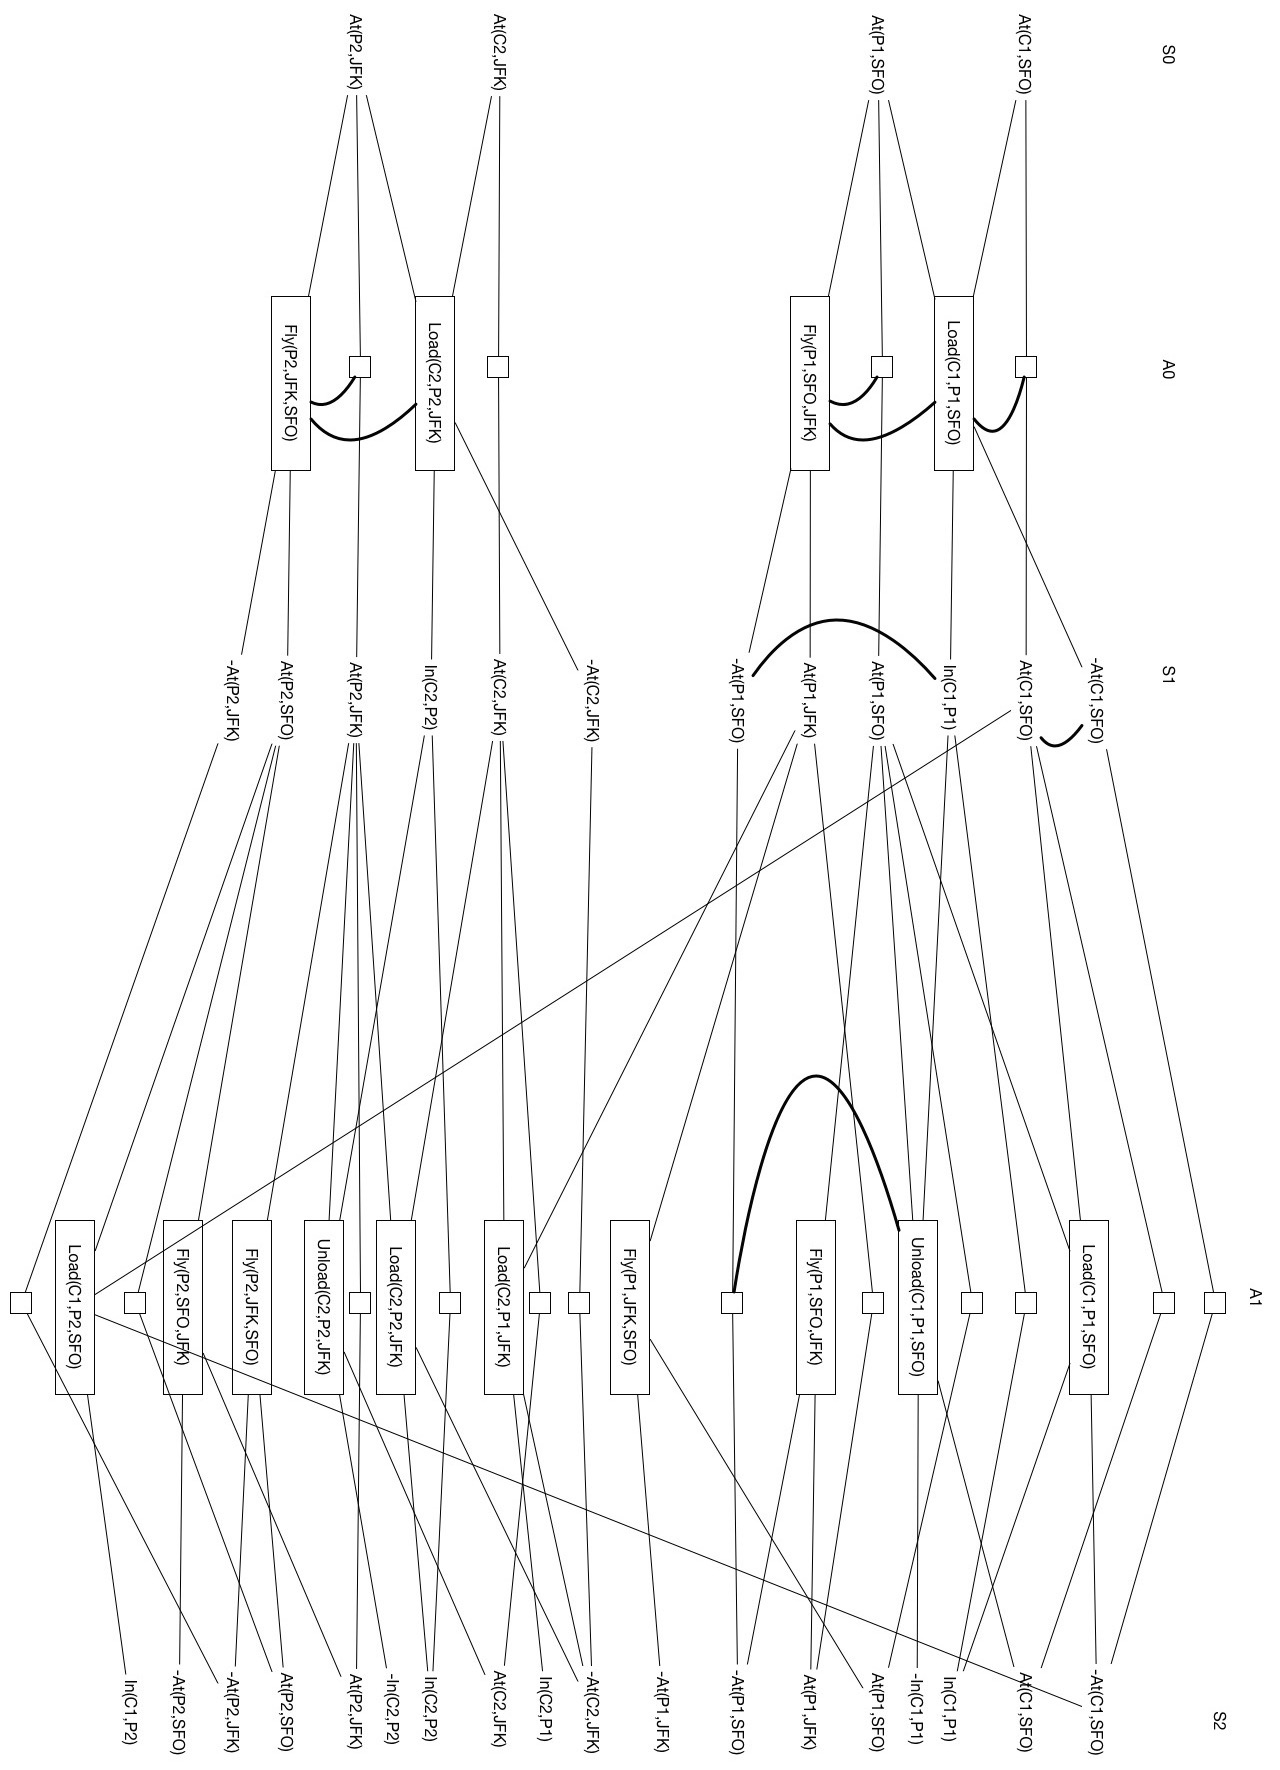
\includegraphics[width=1.0\textwidth]{planninggraph}
	\caption{Ex.3}
	\label{fig:3}
\end{figure}


\section*{Ex.4}
\begin{lstlisting}[mathescape=true]
Primitive actions where t is truck and l is load:
Forward(t);
TurnLeft(t);
TurnRight(t);
Load(l,t)
Unload(l,t)

We have the following high level actions in the grid map with 
x and y as start and a and b as destination:
Move(t, x, y);
Transport(l, t, x, y, a, b);

Refinements:
Transport(l,t,x,y,a,b)
    PRECOND: Truck(t) AND Load(l) AND At(l,x,y)
    STEPS: Move(t,x,y), Load(l,t), Move(t,a,b), Unload(l,t)

Move(t,x,y)
    PRECOND: Truck(t) AND At(t,x,y)
    STEPS:

Move(t,x,y)
    PRECOND: Truck(t)
    STEPS: Forward(t)
    
Move(t,x,y)
    PRECOND: Truck(t)
    STEPS: TurnLeft(t)
    
Move(t,x,y)
    PRECOND: Truck(t)
    STEPS: TurnRight(t)
\end{lstlisting}

\section*{Ex.5}

We need an action which has an effect that is dependant on the evaluation of a condition (like in if-statements from programming languages).

\begin{lstlisting}[mathescape=true]
Move(b,x,y)
    PRECOND: On(b,c) AND Clear(b) AND Clear(y)
    EFFECTS: if y!=Table 
                Then On(b,y) AND Clear(x) AND $\neg On(b,x)$ AND $\neg Clear(y)$
            else
                On(b,y) AND Clear(x) AND $\neg On(b,x)$
\end{lstlisting}

\section*{Ex.6}

a)
\begin{lstlisting}[mathescape=true]
Drink(p)
    PRECOND: Patient(p)
    EFFECTS: $\neg Dehydrated(p)$
    
Medicate(p)
    PRECOND: Patient(p) AND Disease(D)
    EFFECTS: if(has(p,D)) 
                then Cured(p)
            else
                SideEffect(p)
                

\end{lstlisting}

\begin{figure}[ht]
	\centering
  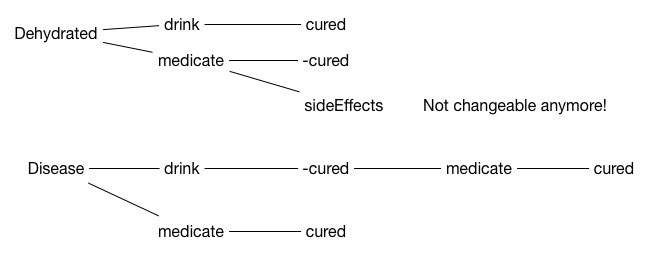
\includegraphics[width=1\textwidth]{6a}
	\caption{Since we cannot remove the side effects, we do not continue the top path}
	\label{fig:6a}
\end{figure}

b)

\begin{figure}[ht]
	\centering
  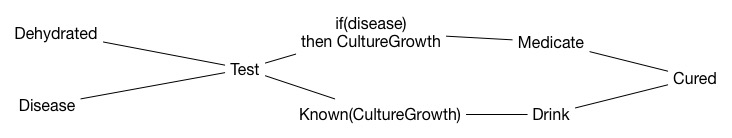
\includegraphics[width=1\textwidth]{6a(2)}
	\caption{Conditional plan that solves the problem}
	\label{fig:6a(2)}
\end{figure}
\end{document}